\documentclass[aps,prb,twocolumn,superscriptaddress,floatfix,longbibliography]{revtex4-2}

\usepackage[utf8]{inputenc}
\usepackage[spanish]{babel}
\usepackage{graphicx}
\usepackage{amsmath}
\usepackage{subcaption}
\usepackage{wrapfig} 
\usepackage[export]{adjustbox}

\usepackage{amsmath,amssymb} % math symbols
\usepackage{bm} % bold math font
\usepackage{graphicx} % for figures
\usepackage{comment} % allows block comments
\usepackage{textcomp} % This package is just to give the text quote '
%\usepackage{ulem} % allows strikeout text, e.g. \sout{text}

\usepackage[spanish]{babel}

\usepackage{enumitem}
\setlist{noitemsep,leftmargin=*,topsep=0pt,parsep=0pt}

\usepackage{xcolor} % \textcolor{red}{text} will be red for notes
\definecolor{lightgray}{gray}{0.6}
\definecolor{medgray}{gray}{0.4}

\usepackage{hyperref}
\hypersetup{
colorlinks=true,
urlcolor= blue,
citecolor=blue,
linkcolor= blue,
bookmarks=true,
bookmarksopen=false,
}

% Code to add paragraph numbers and titles
\newif\ifptitle
\newif\ifpnumber
\newcounter{para}
\newcommand\ptitle[1]{\par\refstepcounter{para}
{\ifpnumber{\noindent\textcolor{lightgray}{\textbf{\thepara}}\indent}\fi}
{\ifptitle{\textbf{[{#1}]}}\fi}}
\ptitletrue  % comment this line to hide paragraph titles
\pnumbertrue  % comment this line to hide paragraph numbers

% minimum font size for figures
\newcommand{\minfont}{6}

% Uncomment this line if you prefer your vectors to appear as bold letters.
% By default they will appear with arrows over them.
% \renewcommand{\vec}[1]{\bm{#1}}

%Cambiar Cuadros por Tablas y lista de...
%\renewcommand{\listtablename}{Índice de tablas}
\renewcommand{\tablename}{Tabla}
\renewcommand{\date}{Fecha}

\usepackage[bottom]{footmisc} %para que las notas al pie aparezcan en la misma página



\begin{comment}

%Comandos de interés:

* Para ordenar el documento:
\section{Introducción}
\section{\label{sec:Formatting}Formatting} %label para luego hacer referencia a esa sección

\ptitle{Start writing while you experiment} %pone nombre y título al documento dependiendo de si en el header están los comandos \ptitletrue y \pnumbertrue

* Ecuaciones:
\begin{equation}
a^2+b^2=c^2 \,.
\label{eqn:Pythagoras}
\end{equation}

* Conjunto de ecuaciones:
\begin{eqnarray}
\label{eqn:diagonal}
\nonumber d & = & \sqrt{a^2 + b^2 + c^2} \\
& = & \sqrt{3^2+4^2+12^2} = 13
\end{eqnarray}

* Para hacer items / enumerar:
\begin{enumerate}
  \item
\end{enumerate}

\begin{itemize}
  \item
\end{itemize}

* Figuras:
\begin{figure}[h]
    \includegraphics[clip=true,width=\columnwidth]{pixel-compare}
    \caption{}
     \label{fig:pixels}
\end{figure}

* Conjunto de figuras:
(no recuerdo)


* Para hacer referencias a fórmulas, tablas, secciones, ... dentro del documento:
\ref{tab:spacing}

* Para citar
Elementos de .bib
\cite{WhitesidesAdvMat2004}
url
\url{http://www.mendeley.com/}\\

* Agradecimientos:
\begin{acknowledgments}
We acknowledge advice from Jessie Zhang and Harry Pirie to produce Fig.\ \ref{fig:pixels}.
\end{acknowledgments}

* Apéndice:
\appendix
\section{\label{app:Mendeley}Mendeley}

* Bibliografía:
\bibliography{Hoffman-example-paper}

\end{comment}

\begin{comment}

Plots y tablas en orden:

* Figura de los cilindros con los PT100, la resistencia de referencia, la fuente, el multímetro y la computadora simbolizando el software de adquisisción de datos.
* Figura de los cilindros con la lampartira, la fuente que le da tensión y el multímetro para medir esa tensión

* Tabla de dimensiones de los cilindros
(la copio de prácticos anteriores)

* Figura del equipo de algto vacío (bomba mecánica, difusora, tubos, bridas, cámara, 3 cilindros...)
* Figura sobre cómo determinar epsilon (pirómetro, termocupla apoyados sobre cilindro exterior sin vacío)

PLOT PPAL:
* T vs t mostrando un gráfico lindo donde se vea bien el transitorio y el estacionario

SUBPLOTS:
* T vs t mostrando qué pasa si hay un cortocircuito interno que hace que la lámpara no prenda (se ven T bajas)
* T vs t mostrando qué pasa si no ponemos el telgopor
* T vs t mostrando qué pasa si falla el vacío
* T vs t mostrando qué pasa en el cilindro externo cuando agregamos N2
* T vs t mostrando qué pasa cuando cambiamos la potencia de la lamparita sobre la marcha



Determinación del producto de ctes
* T vs P recta para calcular la pendiente relacionada con el producto de constantes

Determinación de epsilon
* Gráfico Epsilon vs P

Bibliografía:
* Agregar referencia a la tabla de calibración R vs T
* Agregar referencia a que sacamos los datos de las áreas de un práctico de años anteriores

\end{comment}



\begin{document}

% Allows to rewrite the same title in the supplement
\newcommand{\mytitle}{Agregación limitada por difusión}

\title{\mytitle}

\author{Pablo Chehade \\
    \small \textit{pablo.chehade@ib.edu.ar} \\
    \small \textit{Física computacional, Instituto Balseiro, CNEA-UNCuyo, Bariloche, Argentina} \\}



\begin{abstract}

Se simuló un proceso de agregación limitada por difusión en una red cuadrada con condiciones de borde periódicas y se obtuvo una estructura dentrítica. Se calculó su dimensión fractal a partir de dos definiciones: dimensión de masa y dimensión de box-counting, obteniendo $D_1 = 1.692 \pm 0.003$ y $D_2 = 1.53 \pm 0.03$, respectivamente.

\end{abstract}

\maketitle


\section{Introducción}

Agregación limitada por difusión (DLA por sus siglas en inglés) es un modelo estándar que busca describir el fenómeno de difusión de partículas libres que al entrar en contacto con un agregado (estructura fija), quedan adheridas. De este modo, el agregado crece en tamaño y su estructura queda determinada por la difusión de las partículas, que a nivel microscópico se manifiesta como un random walk, y las interaccciones de las mismas con el agregado. 

Una manera de caracterizar las estructuras resultantes es por medio de la dimensión fractal, la cual generaliza el concepto de dimensión. Si bien existen numerosas definiciones de este concepto, en el presente se considerarán dos de ellas:
\begin{itemize}
    \item Dimensión de masa: sea $M$ la cantidad de partículas (masa) dentro de un círculo de radio $r$ con origen en el centro de la estructura. En un rango intermedio de $r$, dicha cantidad se comporta como $M(r) \, \alpha \, r^{D_1}$, donde $D_1$ es la dimensión de masa.
    \item Dimensión de box counting: sea $N$ la cantidad de cajas de tamaño $d$ necesarias para cubrir la estructura. Su comportamiento en un rango intermedio de $r = 1/d$ es $N(r) \, \alpha \, r^{D_2}$, donde $D_2$ es la dimensión box counting.
\end{itemize}

\section{Método experimental}

Se simuló un DLA con una red cuadrada de tamaño $1024 \times 1024$ y $20000$ partículas. La condición inicial constó de un agregado en el centro formado por una única partícula denominada `semilla' y partículas libres distribuídas al azar en toda la red. En cuanto a la evolución del sistema, se tuvieron en cuenta ciertas consideraciones. En primer lugar, puede haber más de una partícula libre por sitio. En segundo lugar, estas partículas no interactúan entre sí, sino sólo con el agregado. En tercer lugar, una partícula queda adherida al agregado quieto si es primer vecino del mismo. En función de las consideraciones anteriores, la evolución se llevó a cabo del siguiente modo: en cada paso de tiempo todas las partículas libres fueron movidas aleatoriamente a las posiciones vecinas a lo largo de los enlaces de la red. Posteriormente, fueron adheridas al agregado aquellas partículas que estén en contacto con la estructura fija a lo largo de los enlaces de la red y a 45°.

\section{Resultados}

\subsection{Estructura dentrítica}

\begin{figure}[h]
    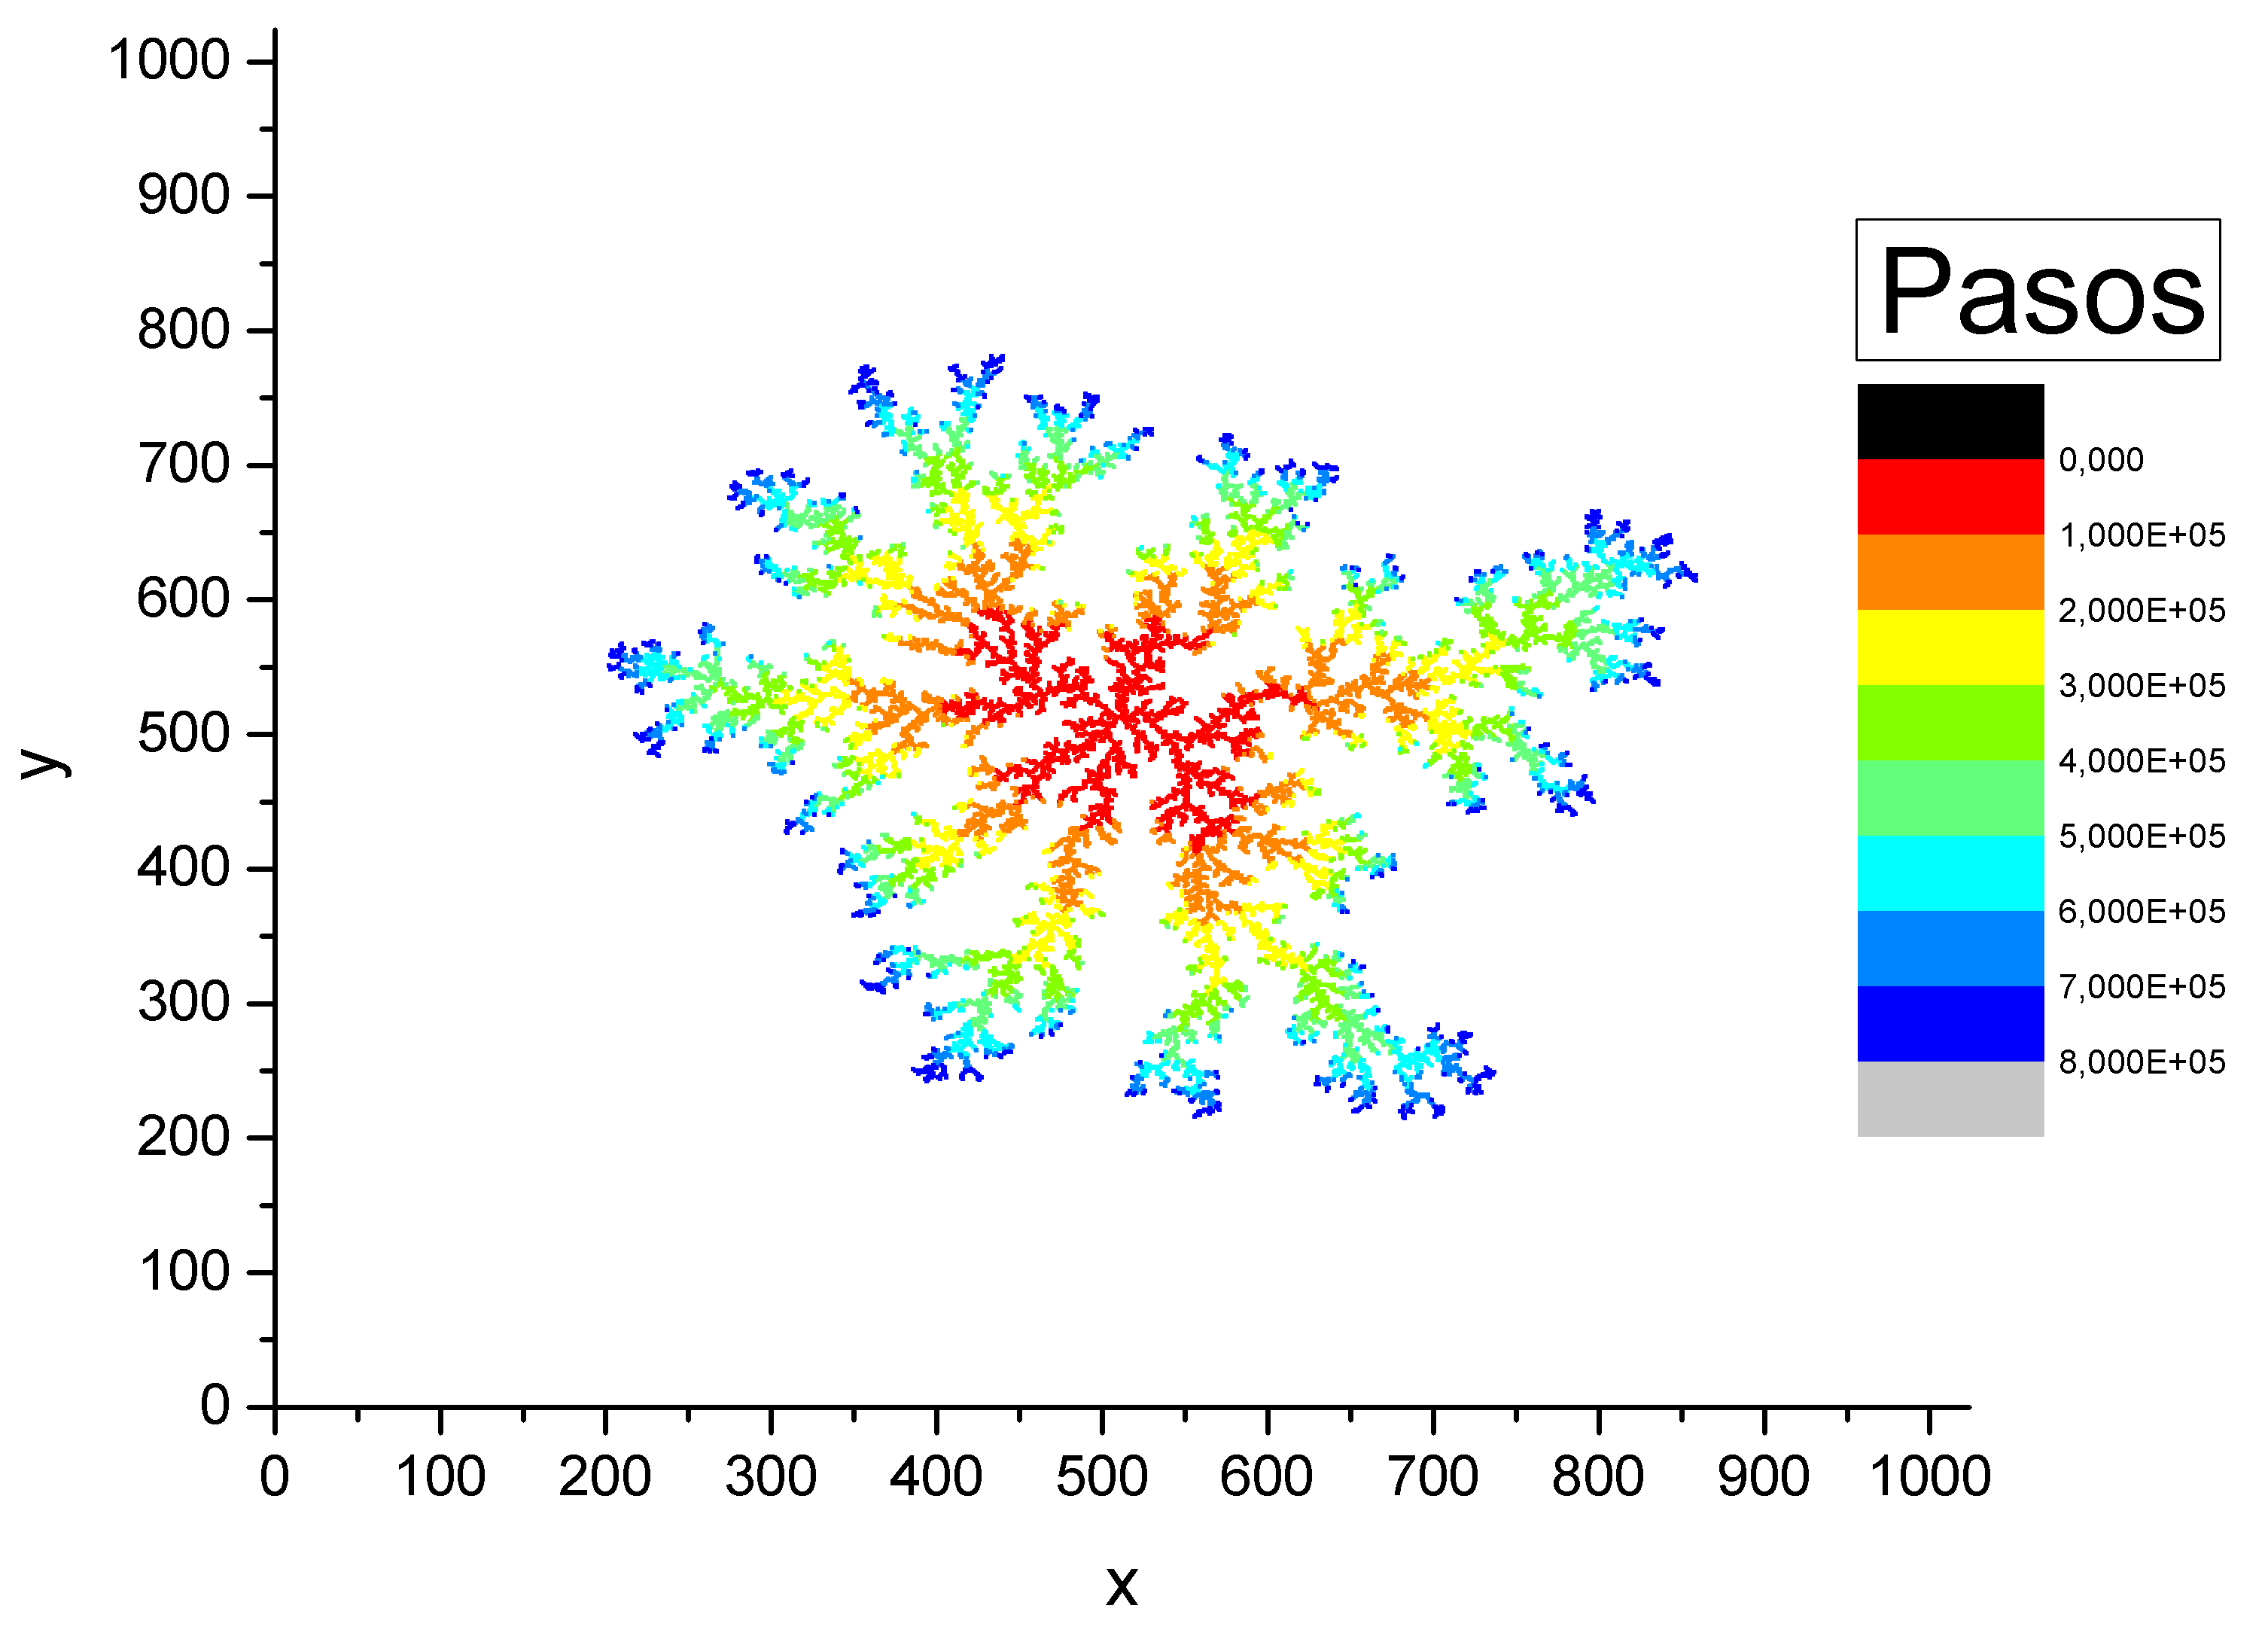
\includegraphics[clip=true,width=\columnwidth]{dendritas.png}
    \caption{Simulación de DLA de $20000$ partículas en una red periódica de $1024 \times 1024$. En colores se indicó en qué paso de tiempo se adhirió cada partícula a la estructura}
     \label{fig:dendritas}
\end{figure}


Luego de $800000$ pasos de tiempo se adhirieron $18522$ partículas. El agregado resultante se grafica en la figura \ref{fig:dendritas}. En colores se indicó en qué paso de tiempo fue adherida cada partícula. Se observa que la estructura crece desde el centro, lo cual concuerda con que la semilla se encuentra en esa posición. Además, la estructura es una dendrita autosemejante que no refleja la geometría de la red que la subyace. También se observa que las partículas se adhieren progresivamente en las ramas exteriores. Esto se justifica en la estructura ramificada de la dentrita: es poco probable que una partícula con movimiento aleatorio llegue al centro de la estructura sin ser atrapada en el camino por alguna de las ramas exteriores. Asimismo, el agregado tiene propiedades geométricas de autosimilaridad e invariancia de escala, propias de los fractales. Sin embargo, a diferencia de los anteriores, estas propiedades dejan de cumplirse en las escalas micro y macro, debido a que se hacen evidentes la discretización de la grilla y el tamaño finito de la estructura, respectivamente. Por último, la estructura no llena completamente el espacio de dos dimensiones, pero lo cubre de una manera peculiar que da cuenta de una dimensión intermedia entre 1 y 2, una dimensión fractal.

\subsection{Dimensión fractal}

\begin{figure}[h]
    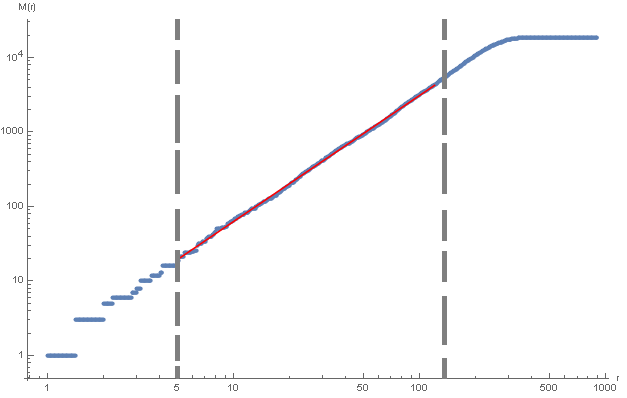
\includegraphics[clip=true,width=\columnwidth]{M(r).png}
    \caption{Cantidad de partículas $M$ dentro de un círculo centrado en la semilla en función del radio $r$ del mismo.}
     \label{fig:M(r)}
\end{figure}

Se procede a calcular las dimensiones fractales $D_1$ y $D_2$ para la dendrita de la figura \ref{fig:dendritas}. En primer lugar, se calculó $M(r)$ para distintos radios. El resultado se grafica en escala ``log-log'' la figura \ref{fig:M(r)}. Se pueden distinguir claramente tres regiones:

\begin{itemize}
    \item $r<5$: el comportamiento es no lineal debido a la discretización de la red. Para valores cercanos a 1 se satura en $M(r) = 1$ correspondiente a la semilla.
    \item $5<r<120$: comportamiento lineal sobre el que aplica la definición de dimensión de masa. En esta región se realizó un ajuste lineal de mínimos cuadrados, cuya pendiente corresponde a $D_1 = 1.692 \pm 0.003$, mayor a 1 y menor que 2.
    \item $r>120$: se hace evidente el tamaño finito de la estructura. Para valores mayores a 500 se produce la saturación de $M(r)$ debido a que la dendrita está completamente contenida.

\end{itemize}

\begin{figure}[h]
    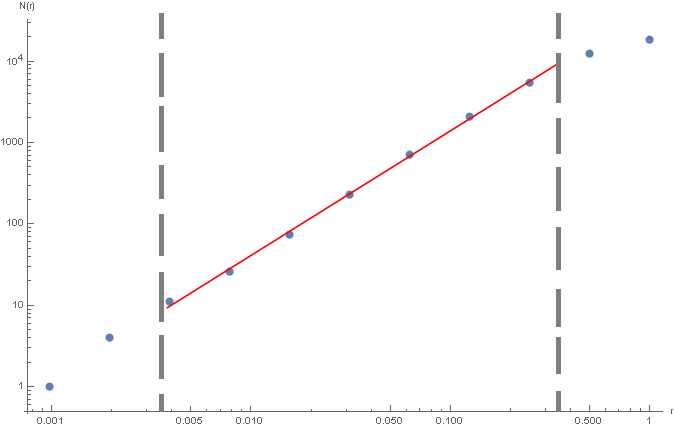
\includegraphics[clip=true,width=\columnwidth]{N(r).png}
    \caption{Cantidad de cajas $N$ necesarias para cubrir la estructura en función de $r = 1/d$, con $d$ tamaño de las cajas.}
     \label{fig:N(r)}
\end{figure}


En segundo lugar, se calculó la cantidad de cajas de tamaño $d$ necesarias para cubrir la estructura. Los valores de $N(r)$ obtenidos con $r = 1/d$ se grafican en la figura \ref{fig:N(r)} en escala ``log-log''. Al igual que $M(r)$, se distinguen tres regiones en el siguiente orden para $r$ creciente: saturación por discretización de la grilla, comportamiento lineal y saturación por tamaño finito de la estructura. En la región lineal se realizó un ajuste de mínimos cuadrados, cuya pendiente es la dimensión fractal $D_2 = 1.53 \pm 0.03$, mayor que 1 y menor que 2. Este valor es distinto a $D_1$ calculado anteriormente. Para que los valores sean idénticos habría que repetir los cálculos anteriores para un ensamble de dentritas. Este proceso no se llevó a cabo debido a que el programa tarda demasiado tiempo en ejecutar.


\bibliography{Radiacion_de_cuerpo_negro}

\end{document}

